%%%%%%%%%%%%%%%%%%%%%%%%%%%%%%%%%%%%%%%%%%%%%%%%%%%%%%%%%%%%%%%%%%%%%
% LaTeX Template: Project Titlepage Modified (v 0.1) by rcx
%
% Original Source: http://www.howtotex.com
% Date: February 2014
% 
% This is a title page template which be used for articles & reports.
% 
% This is the modified version of the original Latex template from
% aforementioned website.
% 
%%%%%%%%%%%%%%%%%%%%%%%%%%%%%%%%%%%%%%%%%%%%%%%%%%%%%%%%%%%%%%%%%%%%%%

\documentclass[11pt]{article}
\usepackage[a4paper]{geometry}
\usepackage[myheadings]{fullpage}
\usepackage{fancyhdr}
\usepackage{lastpage}
\usepackage{graphicx, wrapfig, subcaption, setspace, booktabs}
\usepackage[T1]{fontenc}
\usepackage[font=small, labelfont=bf]{caption}
\usepackage{fourier}
\usepackage[protrusion=true, expansion=true]{microtype}
\usepackage[english]{babel}
\usepackage[nottoc]{tocbibind}
\usepackage{sectsty}
\usepackage{url, lipsum}
\usepackage{hyperref}



\newcommand{\HRule}[1]{\rule{\linewidth}{#1}}
\onehalfspacing
\setcounter{tocdepth}{5}
\setcounter{secnumdepth}{5}

%-------------------------------------------------------------------------------
% HEADER & FOOTER
%-------------------------------------------------------------------------------
\pagestyle{fancy}
\fancyhf{}
\setlength\headheight{15pt}
\fancyhead[L]{Exploring The Work Experiences During COVID-19}
\fancyhead[R]{Survey}
\fancyfoot[R]{Page \thepage\ of \pageref{LastPage}}
%-------------------------------------------------------------------------------
% TITLE PAGE
%-------------------------------------------------------------------------------

\begin{document}

\title{ \normalsize \textsc{SWE 4701\\
Software Metrics and Processes}
		\\ [2.0cm]
		\HRule{0.5pt} \\
		\LARGE \textbf{\uppercase{Survey on Exploring The Work Experiences During COVID-19}}
		\HRule{.5pt} \\ [0.5cm]
		\normalsize  \vspace*{5\baselineskip}}

\date{}

\author{
        Fahim Arsad Nafis\\
        Shah Eftakher Sazid\\
        Saad Bin Johir\\
        Maysha Afrin Munia\\
        Tasnim Jarin Afra\\
        Syeda Mishra Saiara\\
        \\
		Department of Computer Science \& Engineering\\ 
		Program : Software Engineering\\
		Islamic University of Technology, Gazipur, Bangladesh.}

\maketitle
\newpage
%-------------------------------------------------------------------------------
% Section title formatting
%\sectionfont{\scshape}
%-------------------------------------------------------------------------------

%-------------------------------------------------------------------------------
% BODY
%-------------------------------------------------------------------------------
\section*{Contributions}
\begin{center}
\begin{tabular}{ | c | c| c | }
\hline
 \textbf{Student ID} & \textbf{Name} & \textbf{Contributed Fields} \\
 \hline
 170042004 & Fahim Arsad Nafis & Team Communication and Collaboration  \\
 \hline
 170042008 & Shah Eftakher Sazid & Work Experiences and Environment \\ 
 \hline
 170042047 & Saad Bin Johir & Finance \\
 \hline
 170042049 & Maysha Afrin Munia & Work Life Balance \\
 \hline
 170042073 & Tasnim Jarin Afra & Work Experiences and Environment \\
 \hline
 170042077 & Syeda Mishra Saiara & Work Life Balance \\
 \hline
\end{tabular}
\end{center}

\newpage
\tableofcontents
\newpage
\section{Abstract}
COVID 19 pandemic has affected not only our health but also our professional lives as well. The home office has been introduced to a very large extent during the time. As the situation was very new to the world, it needed new measures, new styles to cope. Accomplishing professional tasks staying at home, affected both office performances and personal lives.
We created this survey to learn about the positive and negative outcomes of COVID-19.  We asked professionals in different fields to share their work experiences with us. Going through the collected data, we have found that the majority of the respondents have a negative outlook on their midst-corona work life. In his paper, we have broken down their experiences into categories and analyzed them.

\section{Introduction}
The COVID-19 pandemic changed our lives drastically not only in health hazards but also in professional, corporate, and personal lives. There have been some significant changes in office cultures throughout the world. Based on observed changes, the survey was designed to focus on 4 major parts: i) Team communication and collaboration,  ii) Work-Life balance, iii) Work Experiences and Environment, and iv) Financial Issues. The questionnaires were set according to the relevant subsections that came under the major domains. Further, the analysis was done based on graphical values collected from the data set. In the end, a conclusion was reached describing the choices of our subjects, the numerical analysis, and the insights found.

\section{Methodology}
We conducted a survey of professionals mainly working in the industry. Links to the survey were openly posted in university and professional groups and emailed out to self-identified groups of professionals. The questions selected in this section of the survey were primarily comparison based questions. The absolute scale was measured to map all data.  A total of 141 people completed the survey. 40 of them were students during the time of their employment. 44 had a full-time job and 12 said they were unemployed. Let's look into the subsections of our questions. 

\subsection {Team Communication and Collaboration}
The survey tried to reflect the effectiveness of communication and collaboration with team members and colleagues during the COVID 19 pandemic.
Firstly, we have tried to figure out the communication tools and collaboration tools they have used during their work period. Respondents can choose as many communication applications they have used among Google Workplace, Microsoft Office, Zoom, Skype, Discord or Slack. Respondents are given choices to choose their preferred management and collaboration tools like Jira, Trello, Asana, GitHub, Bitbucket, In-house LMS or ERP systems.

We have also tried to find out how team communication has been affected by the COVID 19 pandemic. The respondents have to choose between 3 options to state their impact - Positively Impacted, Neutral, Negatively Impacted.

We have used a Likert scale from 1 to 10 in order to find out the relation and understanding with the colleagues or team members or fellow mates during the COVID 19.

To ensure contact less communication, remote learning has been greatly introduced during the pandemic. To find out the effectiveness of the remote learning sessions, we have used a Likert scale with a range from 1 to 10.

Work from home has been inspired massively to avoid mass gatherings in workplaces. During this time, a mentionable number of employees have joined. We have tried to figure out the communication and understanding with the newly appointed colleagues or team members or fellow mates using a Likert scale.


\subsection {Work-Life Balance}
Out of the 9 questions asked in this section, 8 were Multiple Choice Questions and 1 was a Likert scale 1 - 10 question. Most MCQs were based on many attributes of a healthy lifestyle and how much professionals deviated from it.  They were asked about the changes made due to COVID-19 and how they coped with it. They were asked about their sleep cycles, week-day schedules, physical and mental health challenges and effects on their personal life and relationships. 

We set the questions back because pandemics changed our lifestyles in a different way that was never experienced before. Work from home or a mixed system in-office hours created differences in regular routines and personal lives. 
Additionally, there were changes in office cultures too regarding the office load distribution or time balance. Many companies gave the flexibility to work at any 9 hours or 8 hours during the day, or they thought it would be okay to work outside the office time since everyone was “at home” during the work from home time.

Thus everything caused a change in personal and work-life balance. It affected the sleep cycle. And time management is affected not only physically but also mentally both in positive and negative ways.

\subsection {Work Experience and Environment}

COVID-19 had a severe impact on the regular work environment thus creating an entirely new working experience. With the introduction of the work from the home paradigm, the workers experienced some drastic changes in their regular work lives. To understand how this affected the workers we designed this section of the questionnaire.

As some of the organizations maintained working in office even during the pandemic, so we had to get the percentage of the working population following the available paradigms, i.e. in office, Work from home and a mixed paradigm of the first two. 
In the case of the population working in the office and mixed paradigm, there was a concern of health. So we wanted to know what percentage of the organizations maintained Covid-19 safety protocols. Also, this group of the population had to travel to their office during this period, we wanted to know about the percentage of organizations providing transportation facilities to the employees. 

As the whole country was in lockdown due to the pandemic so travelling to the office was very difficult. So we wanted to get the idea about the hassle the office goers had to face in this commute. To ensure the health safety and commute hassle of the regular employees some organizations managed accommodation for them. So we wanted to get the percentage of organizations that managed these facilities for their employees.

A new aspect of this pandemic time was work time flexibility. As people were working from home it was very difficult to maintain the traditional work hour. We tried to find out what percentage of the working population had office time flexibility. 

Many employees used to work on the desktop or systems provided by the office. Due to work from home paradigm they no longer had access to the desktop in their office. In such a scenario, we tried to find out how the situation was managed. 
As the new working paradigms had flexible work times and different expectations from the management, there must have been some changes in regular work pressure. So we wanted to get an idea about the new work pressure they are facing.

The organizations have a culture of extra-curricular activities and social events. We wanted to know if they maintained these events during the pandemic.

During this pandemic having a daily meal in a restaurant was not an option. So many organizations arranged a dine-in facility for the employees. We tried to find how many had dine-in facilities in their office. Also if they were satisfied with the hygiene of the facility.

For questions with rating of the respondents' experience we have categorized their experience into 3 categories based on their response, e.g. best experience, moderate experience and worst experience for generating results. 

\subsection {Financial}
The most crucial part people faced directly or indirectly was their financial condition. Due to the lockdown commuting to the workplace was tough and as business slid to downfall many reached the verge of losing their jobs.

The earning of a person is usually divided into his/her family so at first, we tried to understand that paradigm. And for this reason, we then wanted to know if it was tough for them to manage it or how well they think they could overcome this obscurity. There are many reasons and factors one's financial condition can be disrupted. So we tried to pinpoint the direct effect of COVID-19 on it. 

Then comes the workplace. The assistance and support the workplace provided play a major role here. The financial assistance and timely remuneration are a blessing at these times of crisis so we tried to find out that. And lastly, the help they had to take as a loan from others to meet their need for survival was the last question in this section to have an overview of the financial condition.


\section{Result}
Out of the 141 data, there had been some analysis based on the 4 major sections of the survey. The results produced some graphical values which led us to come to a constructive conclusion. The numerical discussions were not peripheral only, rather the results included all kinds of in-depth analysis.  

\subsection {Team Communication and Collaboration}
\subsubsection{Communication Applications}
The survey clearly reflects the dominance of Zoom over other teleconference software. Despite being an unpopular software before COVID 19, Zoom has been the leader in post-COVID 19 times. The tendency of using Google Workplace and Microsoft Office suite office is almost similar. As both of these offers a paid enterprise version of services, usage of this software highly depends on the subscription of the organization. People tend to use Discord and Slack as VoIP, instant messaging and digital distribution platforms. Though slack is exclusively used for business communication, a marginal dominance of Discord has been found over Slack. For a long time, Skype was considered to be the most leading teleconference tool for business. A major downfall can be observed in the case of using Skype. Figure: \ref{fig: Communication Applications}

\begin{figure}[!ht]
	\centering
	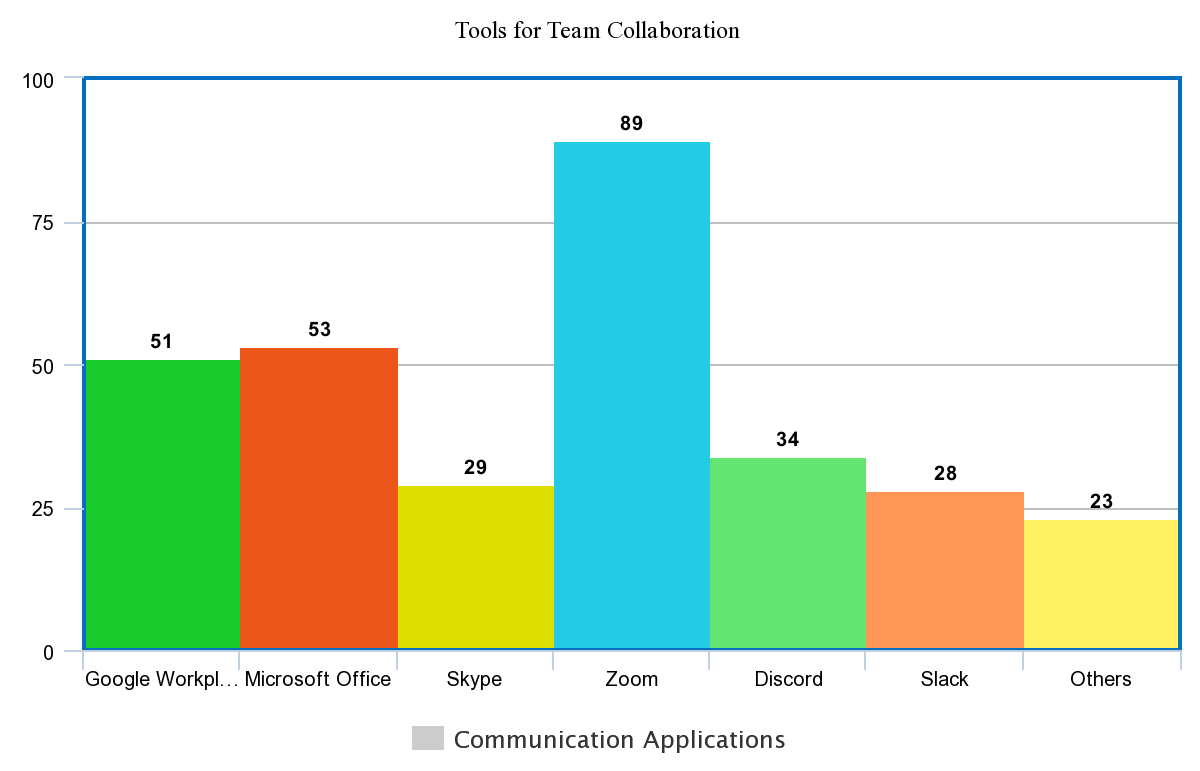
\includegraphics[width=0.8\textwidth]{Images/Collaboration/Communication Tool.png}
	\caption{Usage of Communication Applications during COVID 19}
	\centering
	\label{fig: Communication Applications}
\end{figure}

\subsubsection{Management Applications}
Remote work requires an extensive level of work collaboration. It has been highlighted in the case of task management tools as well. We have noticed the increasing use of management tools during COVID 19. Around 30\% of the total respondents have stated that they have used team organizing, tracking, and task management tools like Trello, Jira, Asana. Besides, almost 39\% of respondents have stated about using version control software like GitHub and Bitbucket. Distributed version control and source code management functionality assist software developers to perform remote jobs more efficiently. Figure: \ref{fig: Management Applications}
\begin{figure}[!ht]
	\centering
	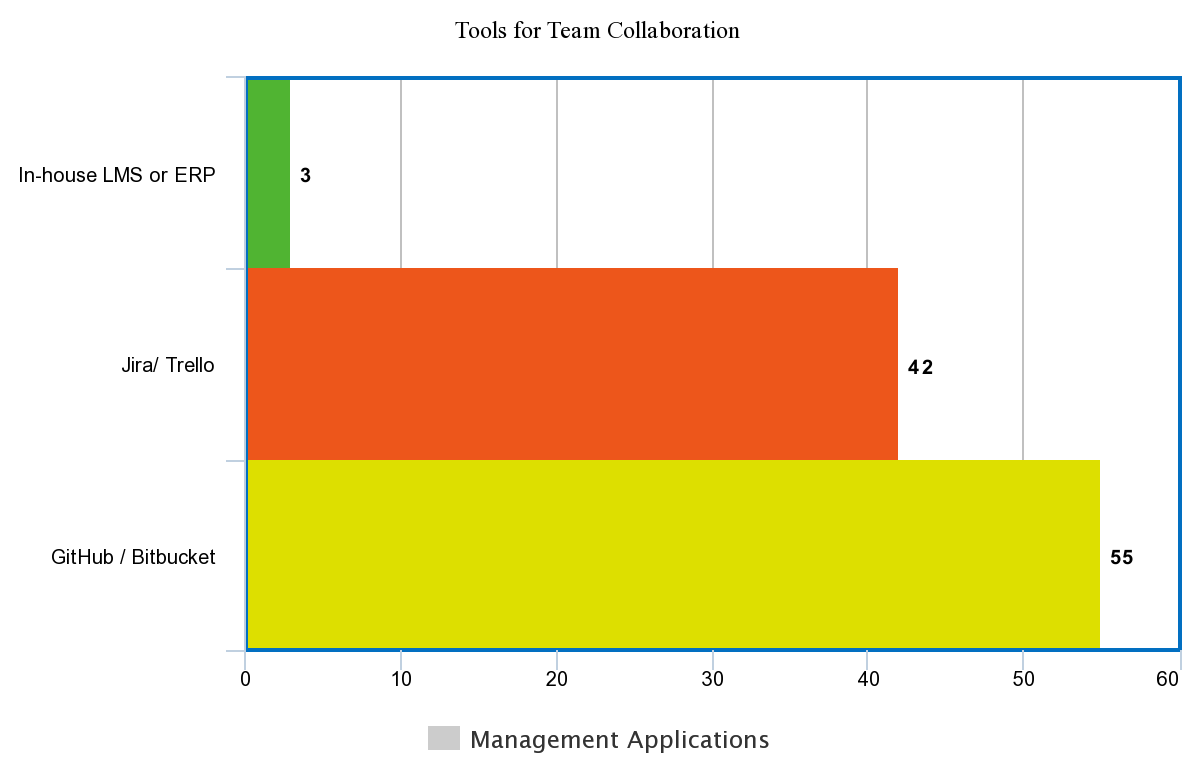
\includegraphics[width=0.8\textwidth]{Images/Collaboration/Management Applications.png}
	\caption{Usage of Management Applications during COVID 19}
	\centering
	\label{fig: Management Applications}
\end{figure}

\subsubsection{ Impact on Team Communication During COVID-19}
The survey reflects that communication and collaboration between colleagues and teammates have been negatively impacted during the outbreak of the COVID 19 pandemic (46.8\%). Remote work and new working strategies have played a huge impact on team communication. A moderate amount of respondents (38.1\%) have been able to cope up with the new normal of the COVID 19 pandemic as team communication has not been affected for them. Around 15.1\% of respondents have claimed to have better understanding and communication between the team members. Figure: \ref{Team Communication}
\newpage
\begin{figure}[!ht]
	\centering
	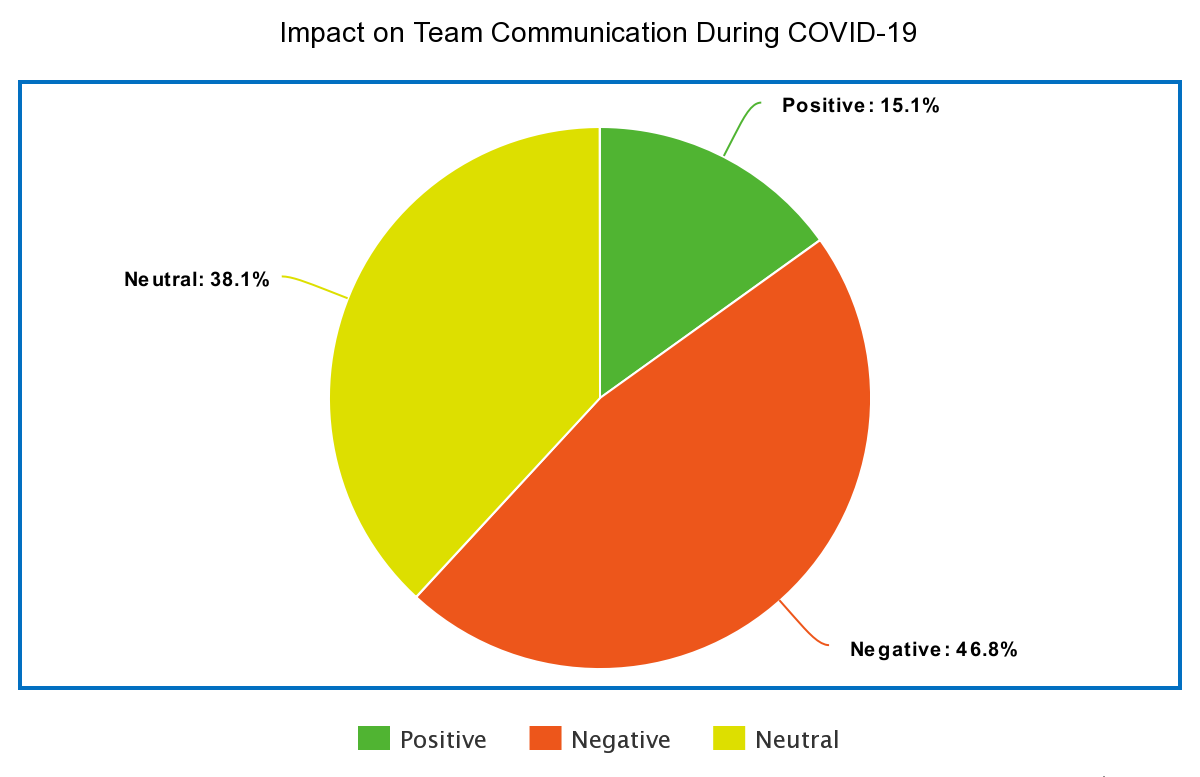
\includegraphics[width=0.8\textwidth]{Images/Collaboration/Team Communication.png}
	\caption{Impact on Team Communication During COVID-19}
	\centering
	\label{Team Communication}
\end{figure}

\subsubsection{Impact on Relation and Understanding with Colleagues}
Relations and understanding between team members and colleagues have been highly affected due to the COVID 19 outbreak. Half of the respondents have reported this negative impact on their team communication. \ref{Relation Colleagues}
\begin{figure}[!ht]
	\centering
	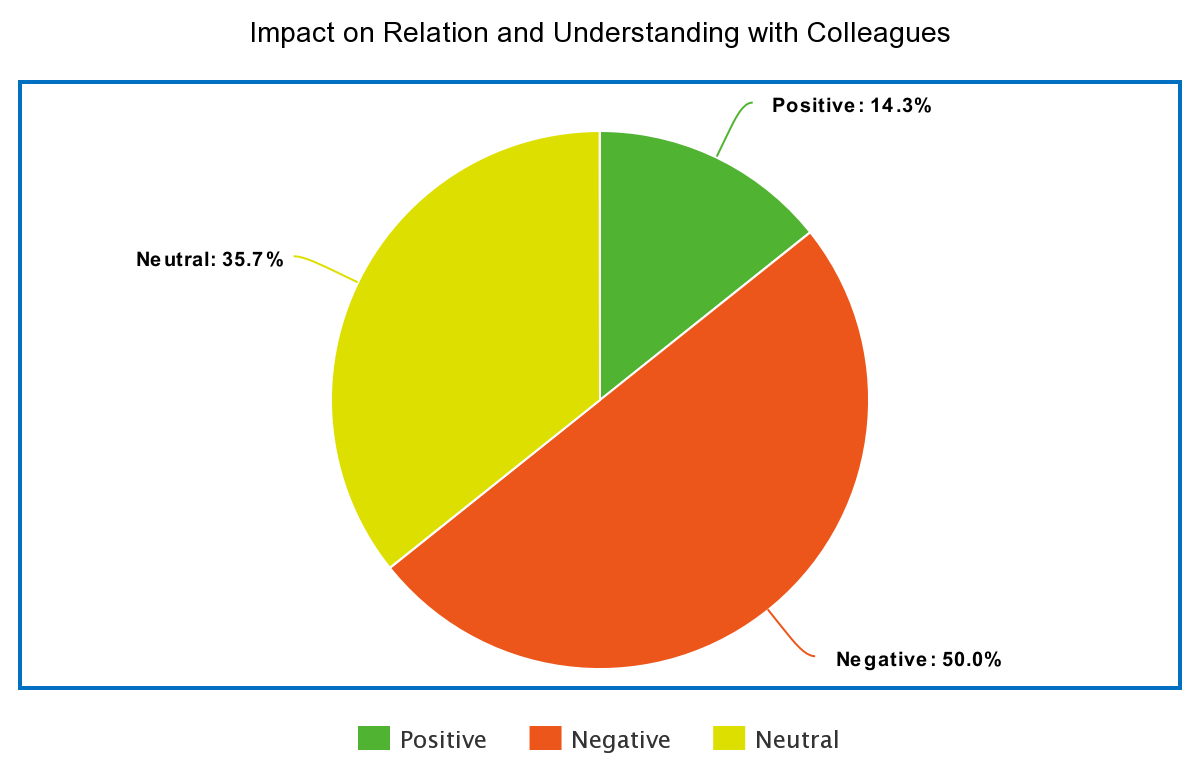
\includegraphics[width=0.8\textwidth]{Images/Collaboration/Relation Colleagues.png}
	\caption{Impact on Relation and Understanding with Colleagues}
	\centering
	\label{Relation Colleagues}
\end{figure}
 35.7\% of people have not noticed any change in relation and understanding with their colleagues. On the other hand, almost the same portion of respondents (14.3\%)  has experienced a positive impact on their understanding of their colleagues. Figure: \ref{Relation Colleagues}

\subsubsection{Effectiveness of Remote Learning Session During COVID 19}
The ineffectiveness of remote learning sessions during COVID 19 has been reflected in the survey. An alarming rate of 64.3\% of respondents has claimed that their remote learning session did not bring any advantage to them. Around 25\% of respondents did not find any difference between live and remote learning sessions. On the contrary, around 10.7\% of respondents have found the remote learning sessions effective and beneficial. Figure: \ref{Remote Learning}
\begin{figure}[!ht]
	\centering
	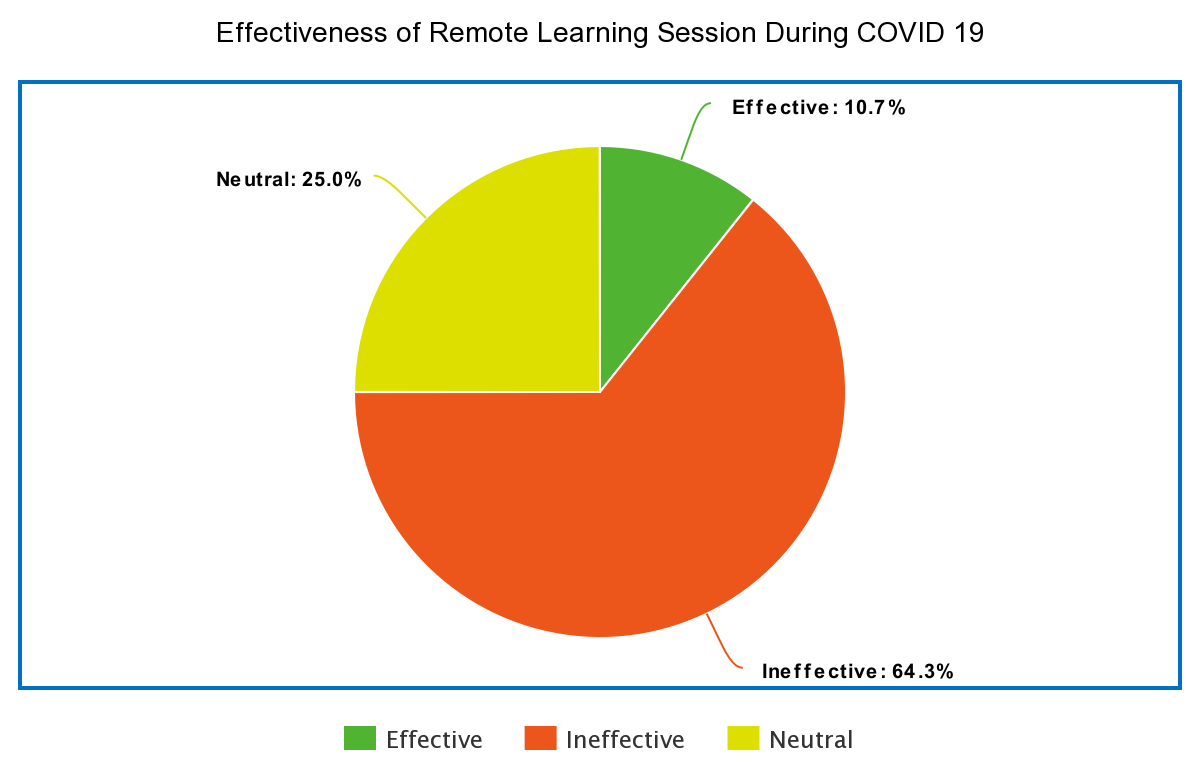
\includegraphics[width=0.8\textwidth]{Images/Collaboration/Remote Learning.png}
	\caption{Effectiveness of Remote Learning Session During COVID 19}
	\centering
	\label{Remote Learning}
\end{figure}

\subsubsection{Impact on Communication with Newly Appointed Employees}
The survey reflects an alarming impact on communication with newly appointed employees during the COVID 19. Around 64.2\% of respondents have raised their concerns regarding the communication gap with their new;y appointed colleagues. Communication with newly joined colleagues seemed normal to around a quarter of the respondents (25.4\%). Around 10.4\% of respondents have developed better communication and relation with newly joined colleagues. Figure: \ref{Newly Appointed Employees}
\begin{figure}[!ht]
	\centering
	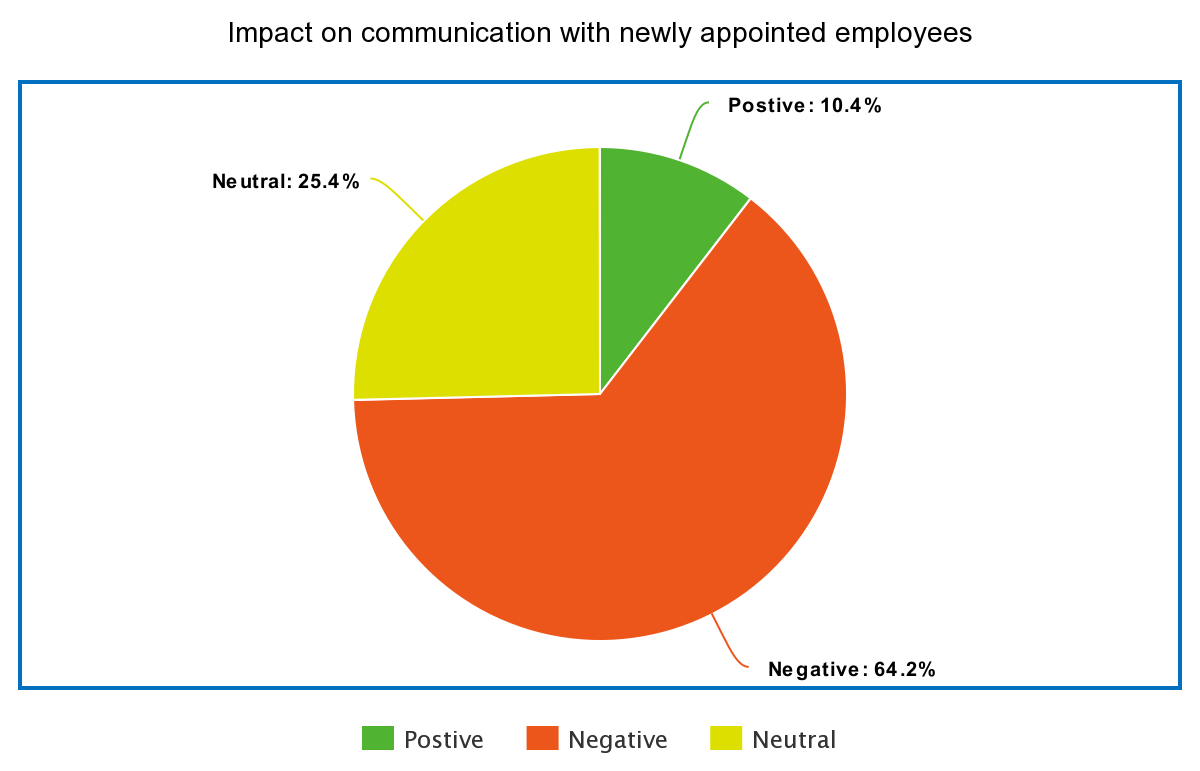
\includegraphics[width=0.8\textwidth]{Images/Collaboration/New Employees.png}
	\caption{Impact on Communication with Newly Appointed Employees}
	\centering
	\label{Newly Appointed Employees}
\end{figure}

\subsection {Work-Life Balance}
\subsubsection{Work Hour Distribution}
38\% of the respondents said that they had to work for more than 40 hours per week during the COVID-19 period. But a similar number, 37\% voted that they worked less than 40 hours. Figure: \ref{Work Hour}
19\% voted that they had to always work outside their scheduled work- hour.  For 20\% this experience was very frequent. Only 9\% agreed that they were not required to work outside their allotted work time. Figure: \ref{Outside Work Hour}
\newpage
\begin{figure}[!ht]
	\centering
	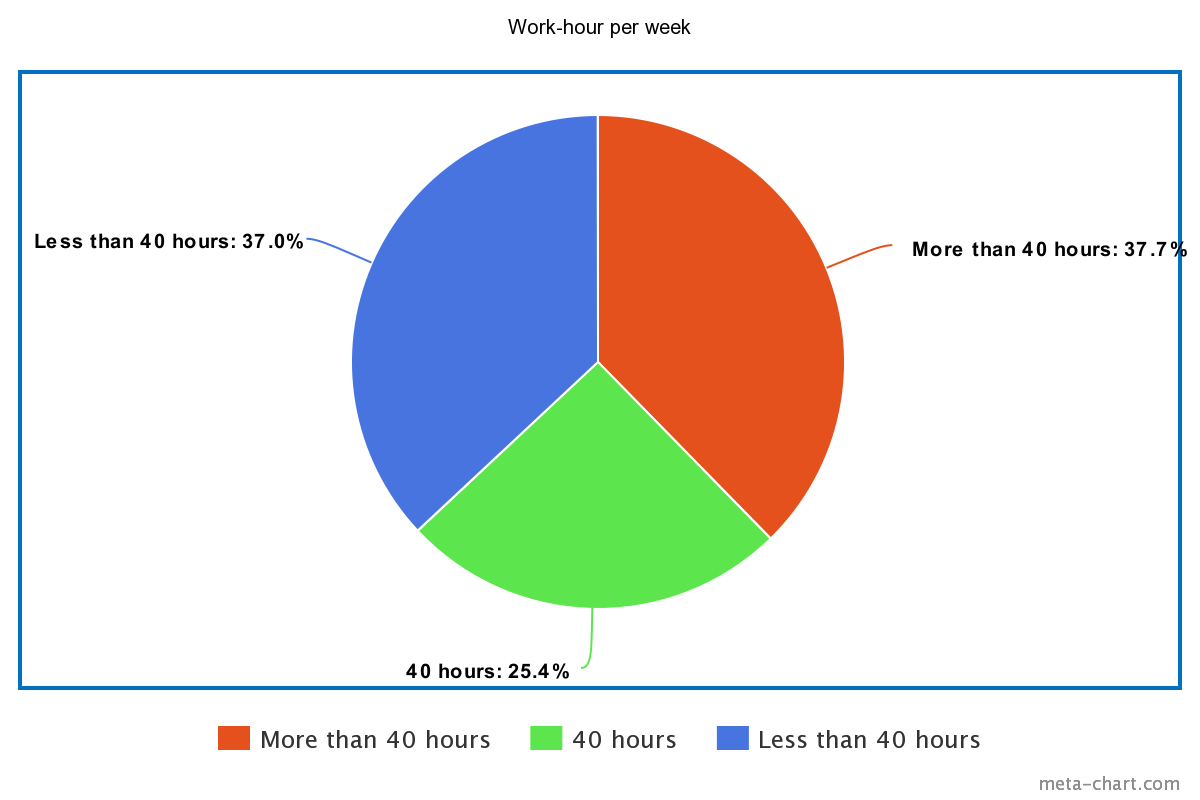
\includegraphics[width=0.8\textwidth]{Images/Work Life/Work Hour.png}
	\caption{Work Hour Distribution during COVID 19}
	\centering
	\label{Work Hour}
\end{figure}
\begin{figure}[!ht]
	\centering
	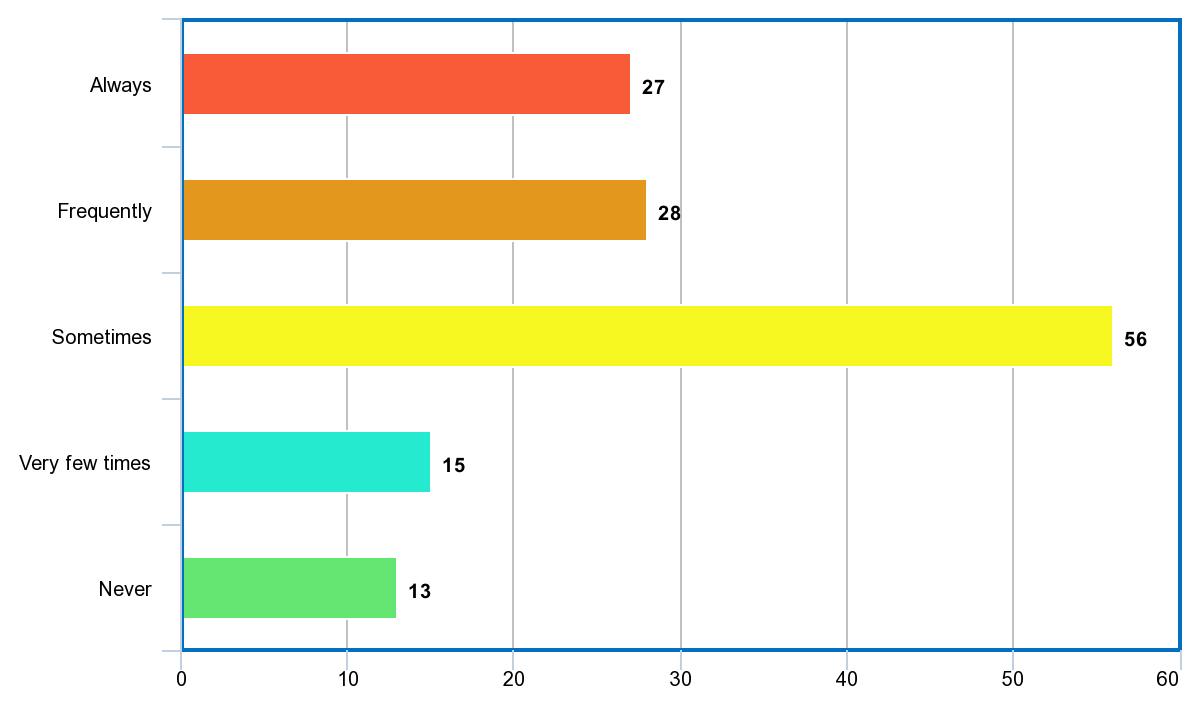
\includegraphics[width=0.8\textwidth]{Images/Work Life/Outside Work Hour.png}
	\caption{Work Outside Work Hour during the COVID-19}
	\centering
	\label{Outside Work Hour}
\end{figure}

\subsubsection{Impact on Health}
71\% of the respondents claim that their sleep schedule has been affected due to the workload. Only 18\% have claimed otherwise. Out of the 141 respondents, 48\% have disclosed facing mental health challenges and 50\% have disclosed facing physical health challenges. Figure: \ref{Impact on Health during COVID 19}
\newpage
\begin{figure}[!ht]
	\centering
	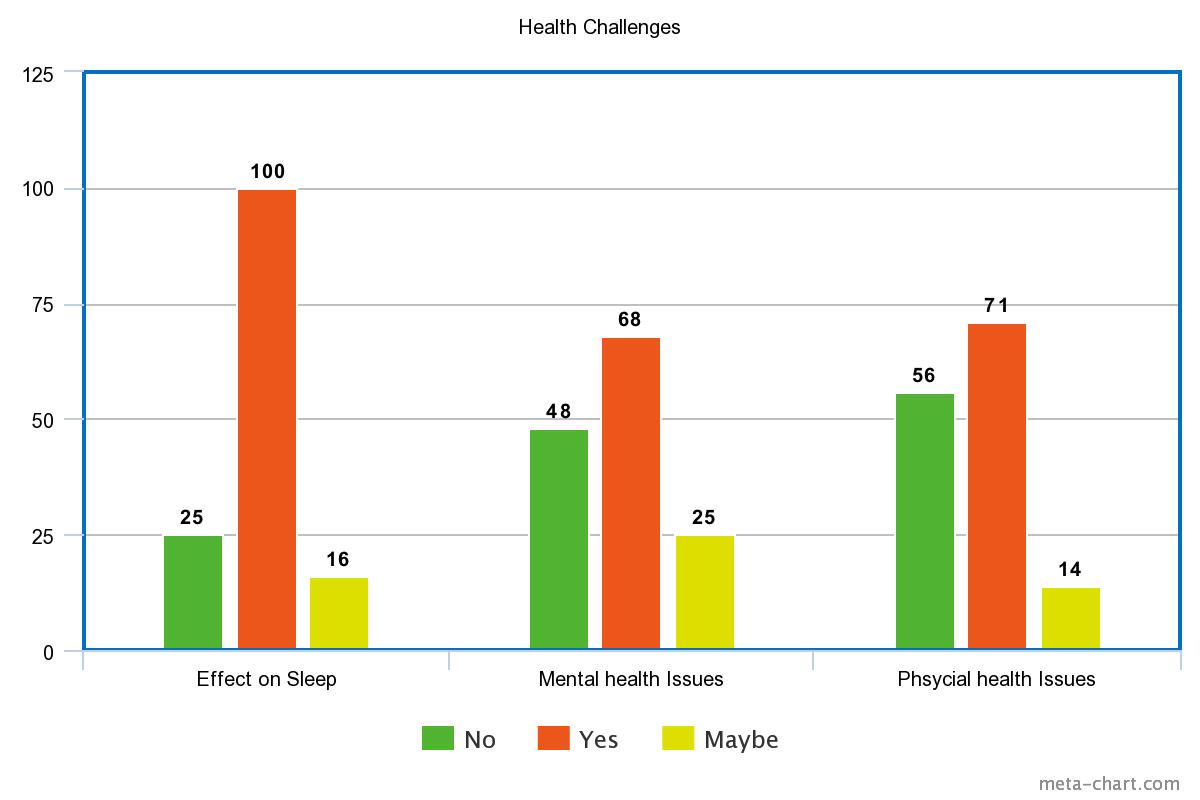
\includegraphics[width=0.8\textwidth]{Images/Work Life/Health Challenges.png}
	\caption{Work Outside Work Hour during the COVID-19}
	\centering
	\label{Impact on Health during COVID 19}
\end{figure}

\subsubsection{Effect on Personal Relationship during Home Office}
Out of the 141 subjects of the survey, the home office significantly affected personal relationships for 33.1\%  of the respondents. For 20.1\%, it affected positively in personal life. And it was the same as before for the rest 46.8\%. Figure: \ref{Effect on Personal Relationship}
\begin{figure}[!ht]
	\centering
	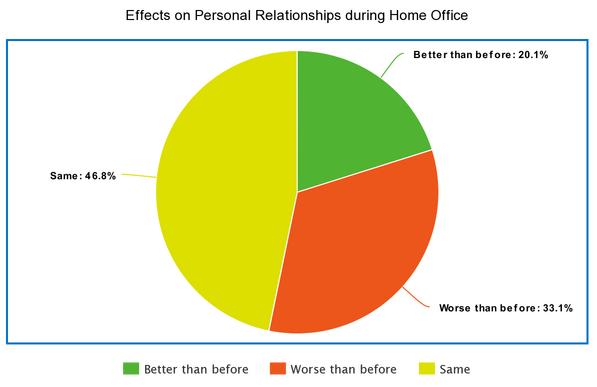
\includegraphics[width=0.8\textwidth]{Images/Work Life/Personal Relations.png}
	\caption{Effect on Personal Relationship during Home Office}
	\centering
	\label{Effect on Personal Relationship}
\end{figure}

\subsubsection{Effects on Overall Work-Life Balance}
71\% of the respondents claim that their sleep schedule has been affected due to the workload. Only 18\% have claimed otherwise. Out of the 141 respondents, 48\% have disclosed facing mental health challenges and 50\% have disclosed facing physical health challenges. Figure: \ref{Effects on Overall Work-Life Balance}
\begin{figure}[!ht]
	\centering
	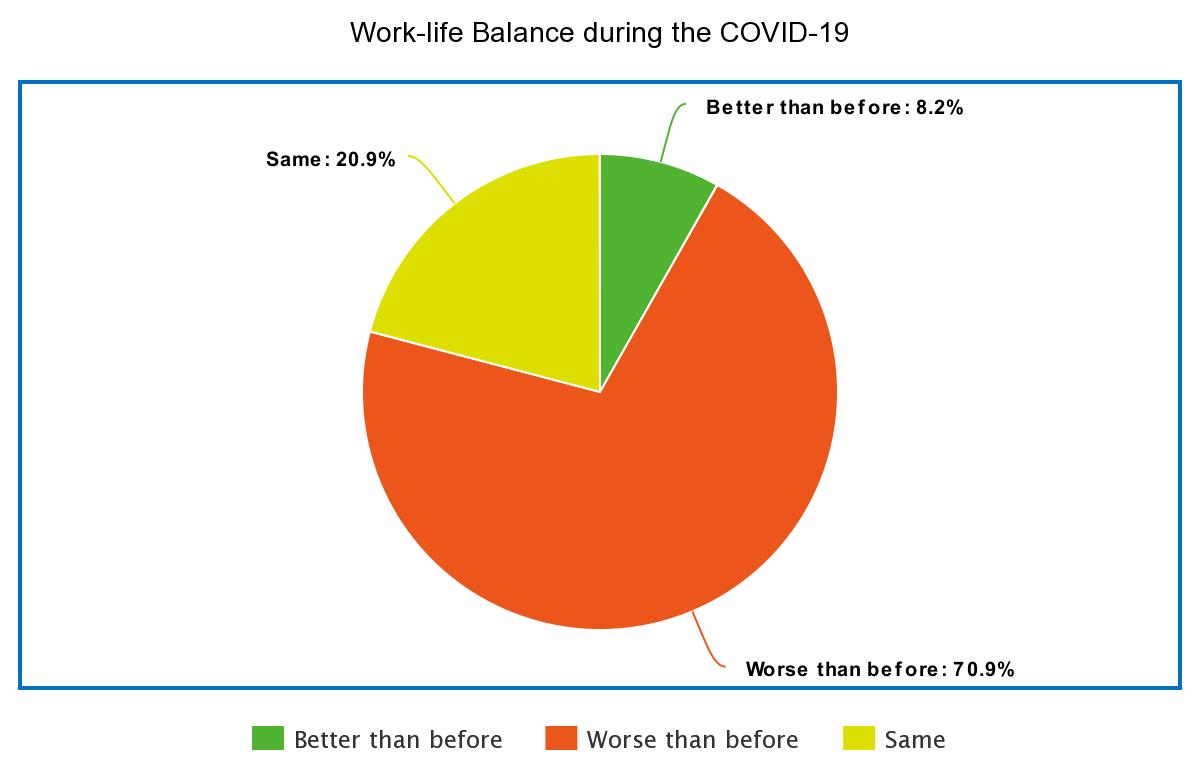
\includegraphics[width=0.8\textwidth]{Images/Work Life/Work Life Balance.png}
	\caption{Effects on Overall Work-Life Balance}
	\centering
	\label{Effects on Overall Work-Life Balance}
\end{figure}


\subsection {Work Experience and Environment}
\subsubsection{Work Paradigm}
From the pie chart in figure \ref{Work parad}, we can see that 50\% of the people worked from home in the time frame from March 2020 to September 2021. Almost 43\% of the respondents worked in a hybrid environment and the rest 7\% had to work completely from the office. From the collected data we can conclude that majority of the office was flexible about their work environment during COVID-19.
\newpage
\begin{figure}[!ht]
	\centering
	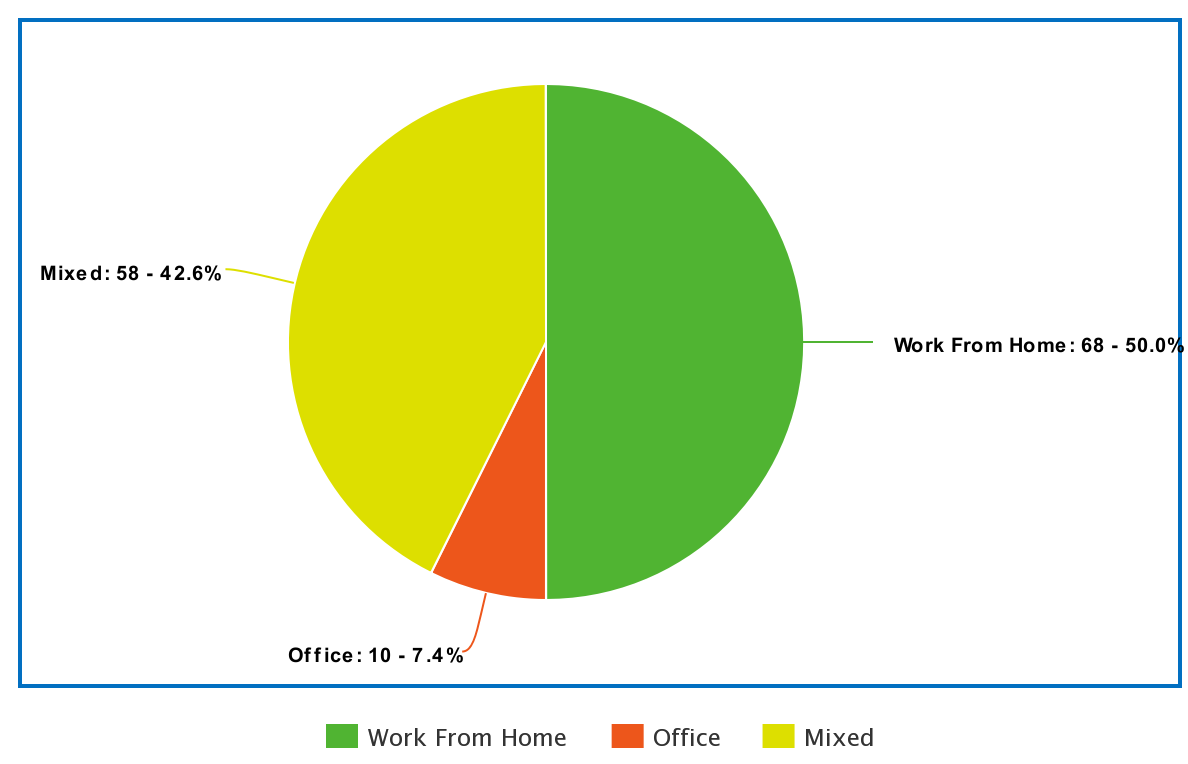
\includegraphics[width=0.8\textwidth]{Images/Experience/Work Paradigm.png}
	\caption{Work paradigms during COVID-19}
	\centering
	\label{Work parad}
\end{figure}


\subsubsection{COVID 19 Health Safety Protocol}
The majority of the respondents who worked from the office mentioned that their workplace maintained health safety protocol as shown in figure \ref{health}. Among them, only 9\% said the other way. It is also seen from the data that 89\% of the people who were dissatisfied with their office maintaining health safety for COVID-19 also had poor work-life balance.

\begin{figure}[!ht]
	\centering
	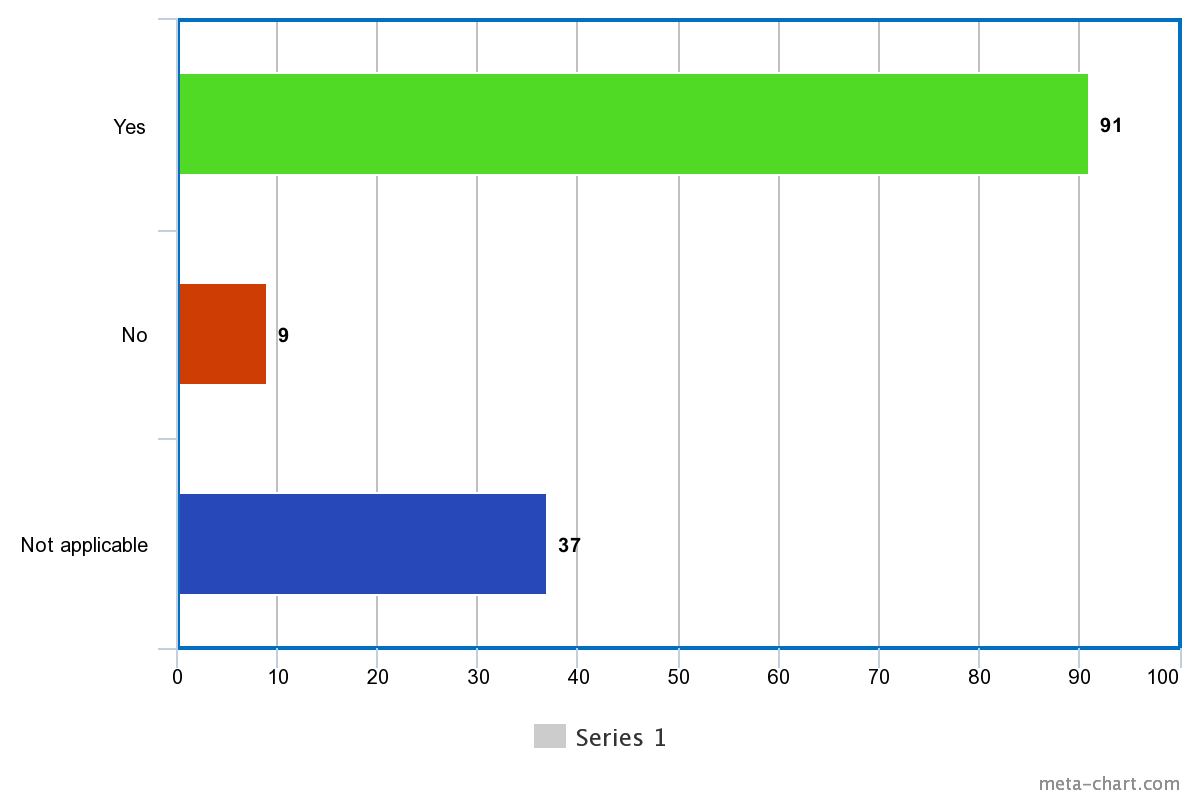
\includegraphics[width=0.8\textwidth, height=2in]{Images/Experience/Health Safety.png}
	\caption{Maintenance of COVID 19 Safety Protocol}
	\centering
	\label{health}
\end{figure}


\subsubsection{Transportation Facilities and Impacts on Commute}
78\% of the people who attended the office said that no transportation was provided from their office according to the finding shown in figure \ref{transport}. Among them, the majority said that they had to face commute hassle while travelling between office and home and had a poor work-life balance. According to figure \ref{commute}, the majority of the regular commuters, 66.4\% expressed that their experience was horrible, where only 12.5\% were satisfied with their daily commute. The rest of them 21.1\% had moderate hassle in their commute. 

\begin{figure}[!ht]
	\centering
	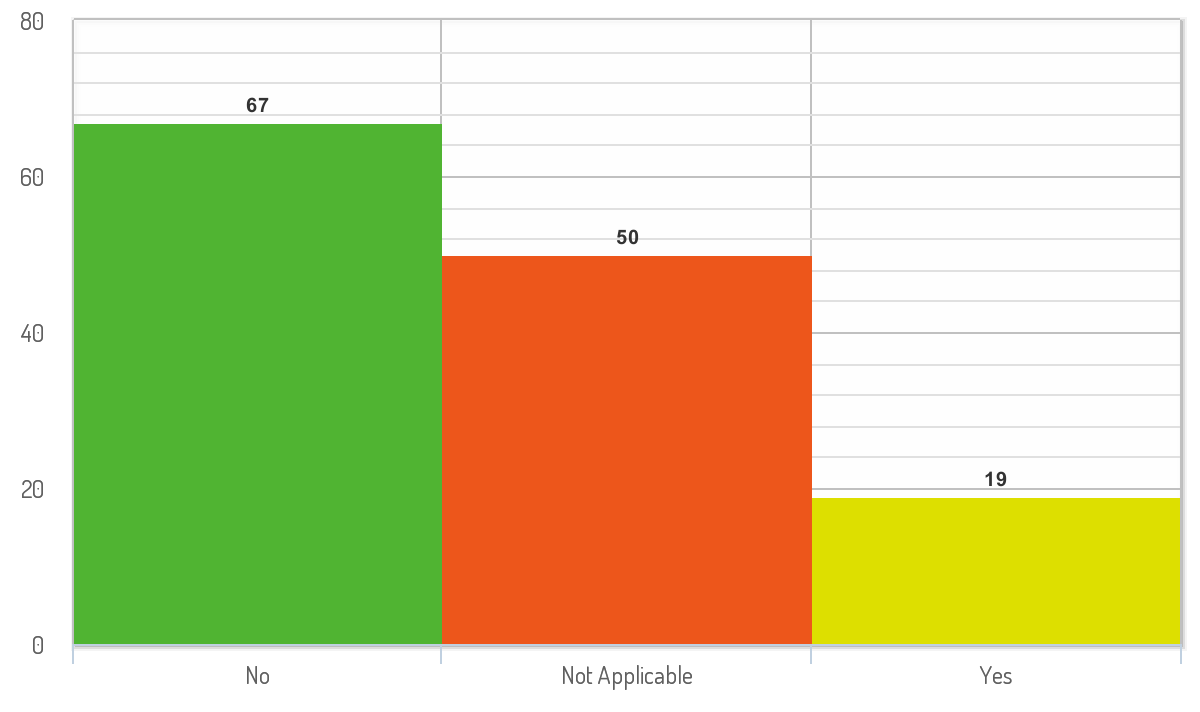
\includegraphics[width=0.8\textwidth]{Images/Experience/Transportation.png}
	\caption{Availability of Transportation}
	\centering
	\label{transport}
\end{figure}


\begin{figure}[!ht]
	\centering
	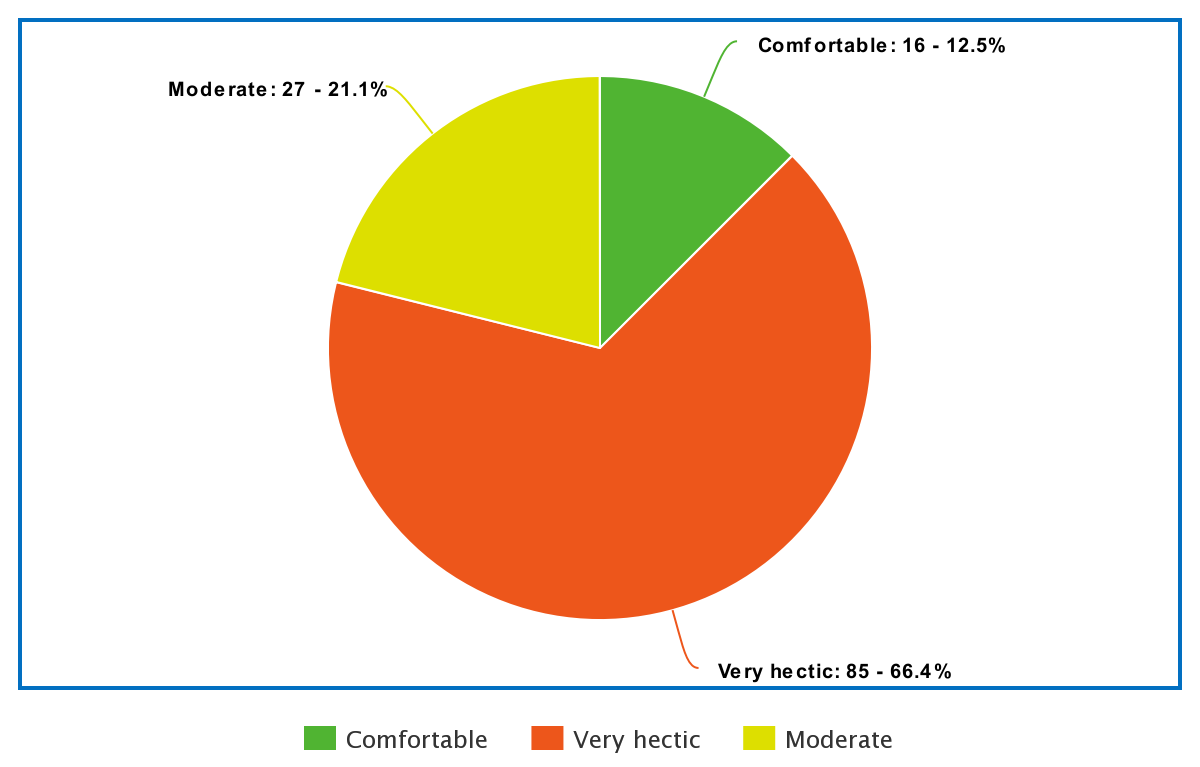
\includegraphics[width=0.8\textwidth]{Images/Experience/commute.png}
	\caption{Communication Hassle}
	\centering
	\label{commute}
\end{figure}


\subsubsection{Residential Accommodation}
From the graph in figure \ref{Accommodation}, we can find that very few of the respondents had residential facilities in their office, about 12.7\%, the rest 87.3\% did not have any residential facility provided by their office.

\begin{figure}[!ht]
	\centering
	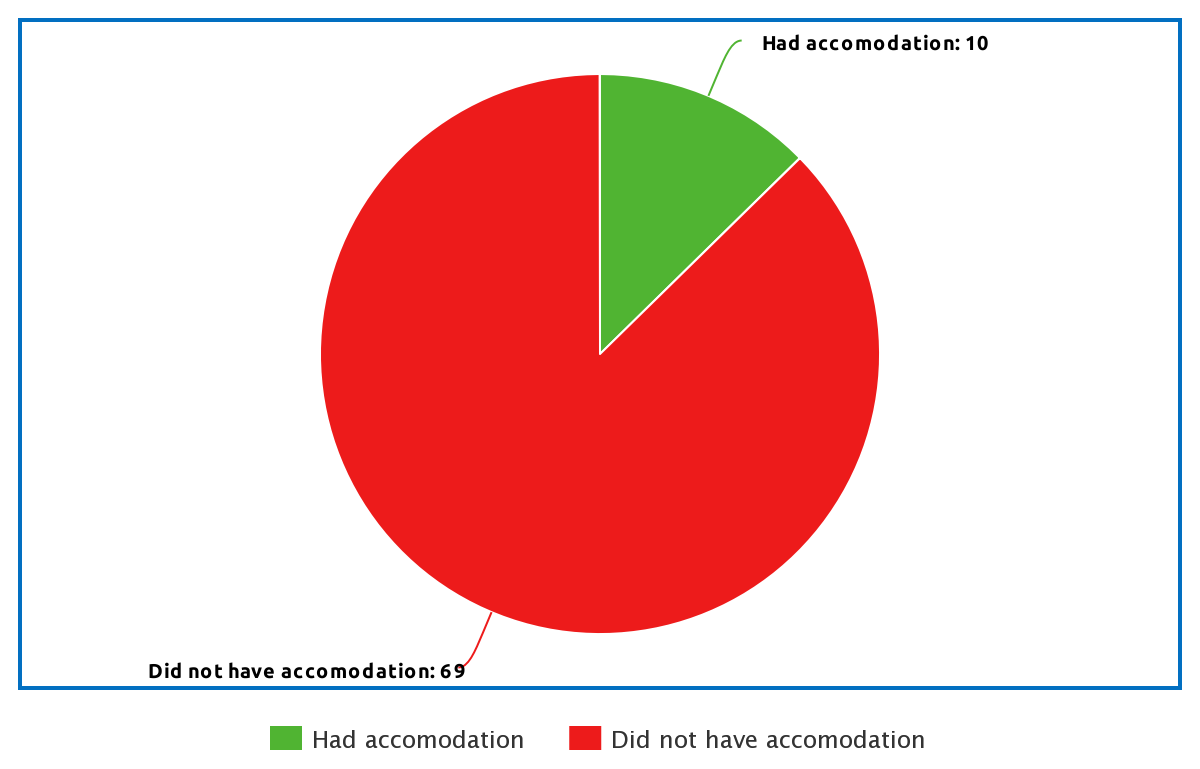
\includegraphics[width=0.8\textwidth]{Images/Experience/Accommodation.png}
	\caption{Accommodation facility}
	\centering
	\label{Accommodation}
\end{figure}

\subsubsection{Office Hour Flexibility}
From the graph in figure \ref{flexibility}, we can see that the majority of the applicable respondents about 75\% had flexible working hours and the rest 25\% did not have any flexible working hours. 
\newpage
\begin{figure}[!ht]
	\centering
	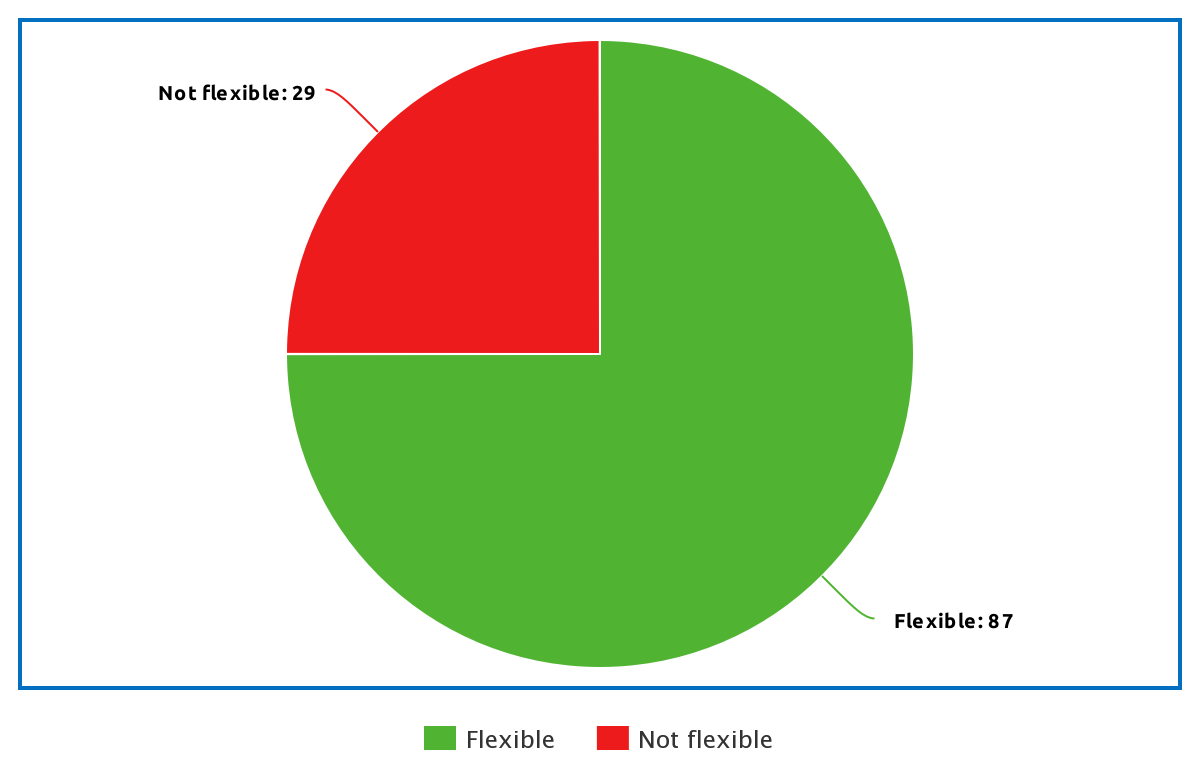
\includegraphics[width=0.8\textwidth]{Images/Experience/flexibility.png}
	\caption{Work hour flexibility}
	\centering
	\label{flexibility}
\end{figure}

\subsubsection{Availability of Work Devices}
From the graph in figure \ref{devices}, we can see that the number of workers with provided devices and working on personal devices is almost similar.  
\begin{figure}[!ht]
	\centering
	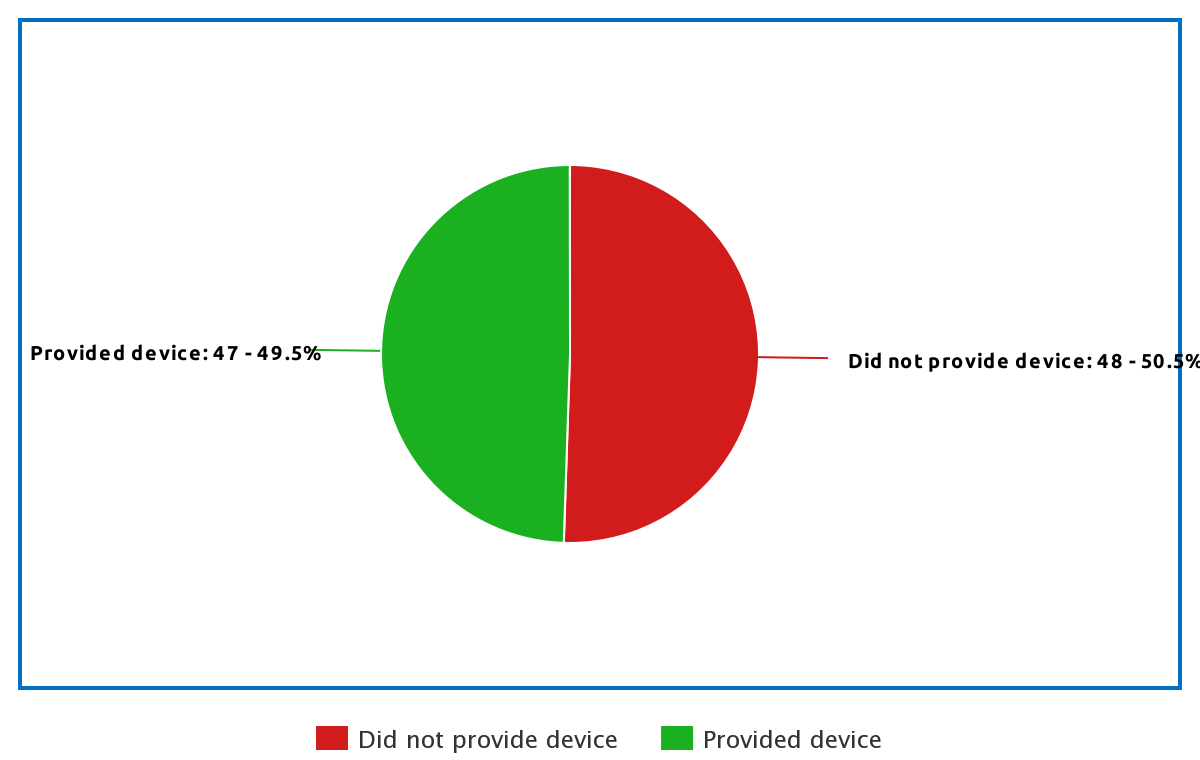
\includegraphics[width=0.8\textwidth]{Images/Experience/devices.png}
	\caption{Provided devices vs personal devices}
	\centering
	\label{devices}
\end{figure}

50.5\% of the applicable respondents did not have their working devices provided by the office and 49.5\% of them had devices provided by their office. Additional data has been found that the majority of the people who had their devices provided by their office, almost 98\% of them were financially secure and did not have to take out loans to get through the pandemic. Moreover, we have found that people who did not get devices from the office had difficulty communicating with new colleagues or team members(Those who have joined during the pandemic). 


\subsubsection{Impact on Work Pressure}
From the work pressure graph in figure \ref{pressure}, we can see that the majority of the respondents’ that is 45.7\%, had moderate work pressure. 35.5\% were satisfied with their work pressure but 18.8\% of the respondents reported that they had extreme work pressure in this pandemic period.

\begin{figure}[!ht]
	\centering
	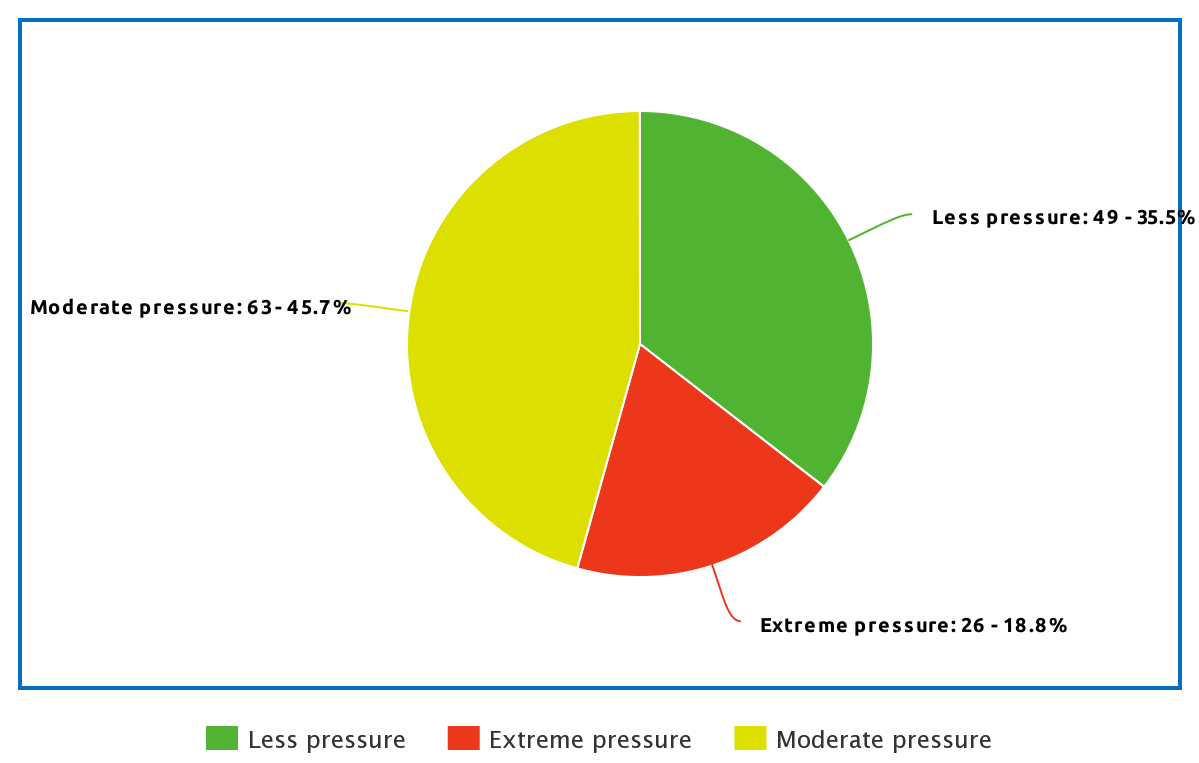
\includegraphics[width=0.8\textwidth]{Images/Experience/work-pressure.png}
	\caption{Work pressure}
	\centering
	\label{pressure}
\end{figure}

\subsubsection{Impact on Extra Curricular and Social Activities}
We can see from the graph in figure \ref{social}, that the majority of the respondents’ organizations stopped all sorts of extra-curricular activities and social events. Out of 111 applicable data, 60.4\% stopped all sorts of extracurricular activities and 39.6\% continued with their extracurricular and social events during this period.
\newpage
\begin{figure}[!ht]
	\centering
	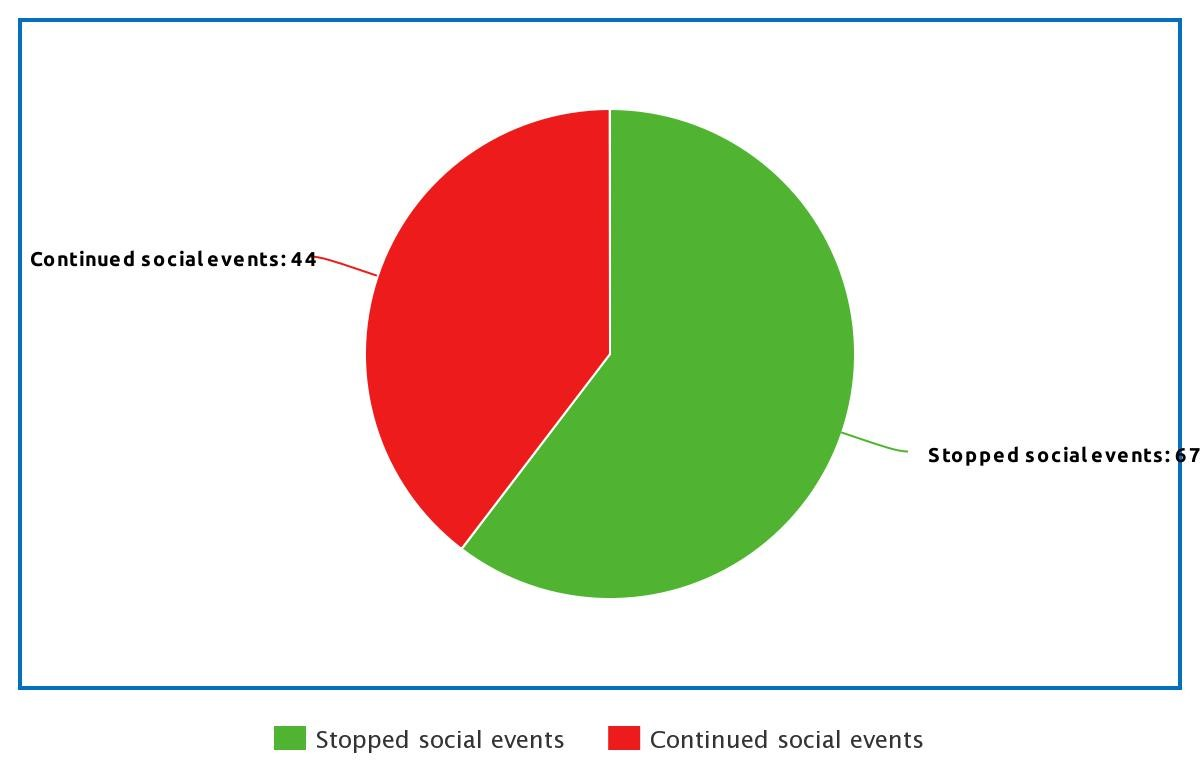
\includegraphics[width=0.8\textwidth]{Images/Experience/social events.jpeg}
	\caption{Impact on Social Events}
	\centering
	\label{social}
\end{figure}

\subsubsection{Dine In Hygiene}
We can see from the figure \ref{dine-in}, a majority of the offices, almost half of the respondents’  offices had a dine-in facility for their employees. 60.4\% of the respondents had a dine-in facility in their office, 39.6\% did not have any dine-in facility in their office. 

\begin{figure}[!ht]
	\centering
	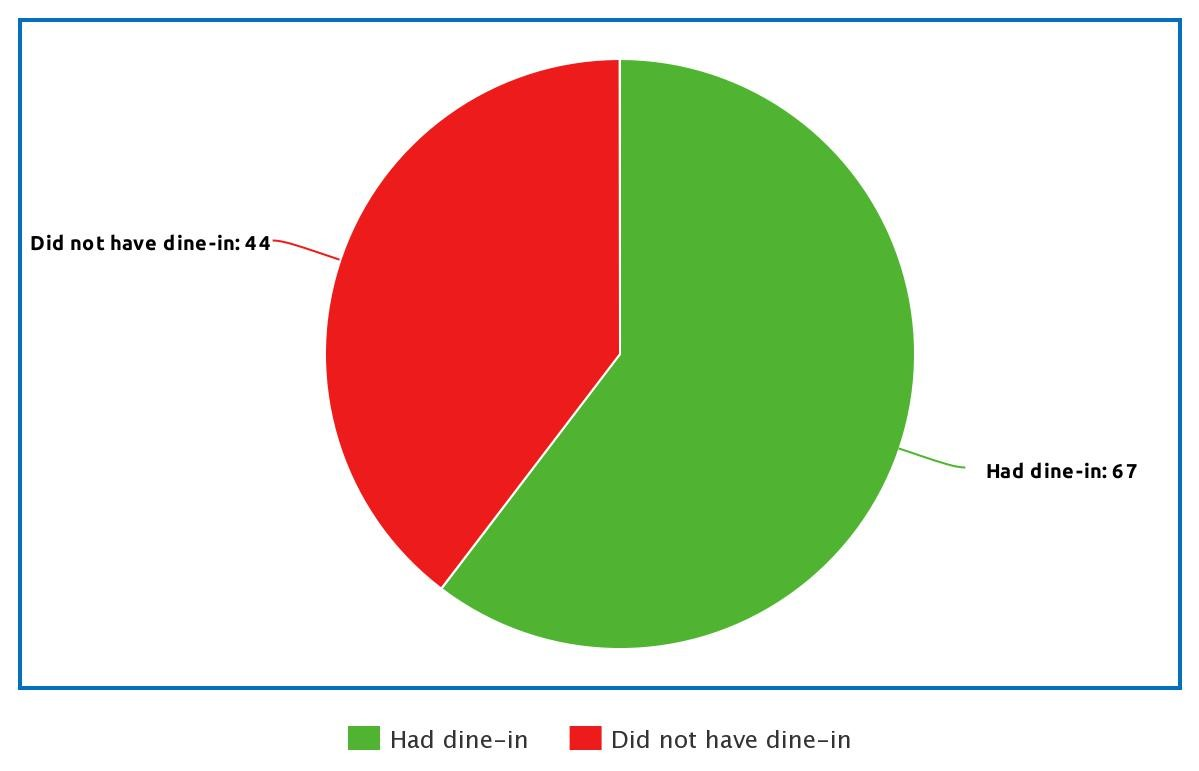
\includegraphics[width=0.8\textwidth]{Images/Experience/dine-in.jpeg}
	\caption{Availability of dine-in facility}
	\centering
	\label{dine-in}
\end{figure}

26\% of the respondents had excellent dine-in facilities in their office. 47\% were satisfied with their dine-in facility and the rest 36.5\% of the respondents had an unhygienic dine-in facility, figure \ref{hygiene}. 

\begin{figure}[!ht]
	\centering
	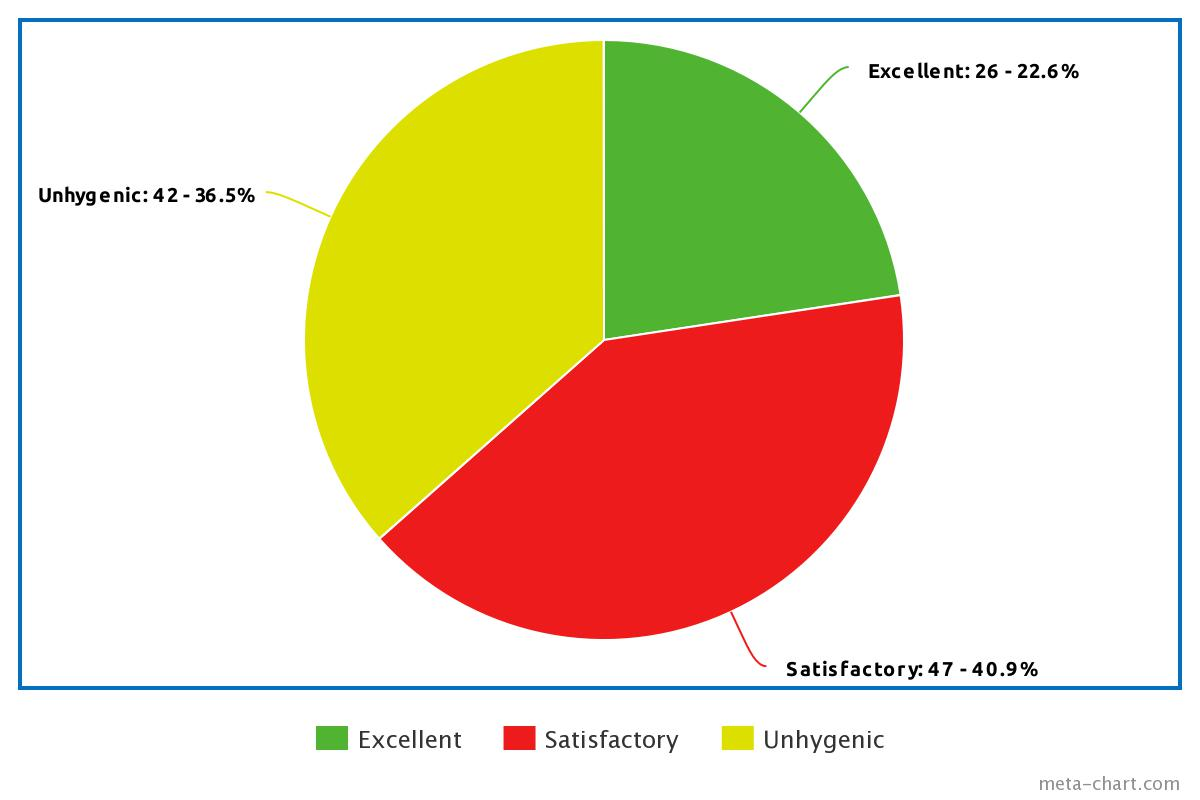
\includegraphics[width=0.8\textwidth]{Images/Experience/hygiene.jpeg}
	\caption{Dine-in hygiene}
	\centering
	\label{hygiene}
\end{figure}

\subsection {Financial}
\subsubsection{Financial Dependency}
From the given chart in the figure \ref{financialDep}, we can see that 73\% of the people had no one dependent on them and 20\% had 1-2 people financially dependent on them and the rest had even more. Hence the data says that most of the people had to only care about themselves and their survival and the rest had to pull off an average of 3 people during this pandemic situation which was rather tough and stressful on them.
\newpage
\begin{figure}[!ht]
	\centering
	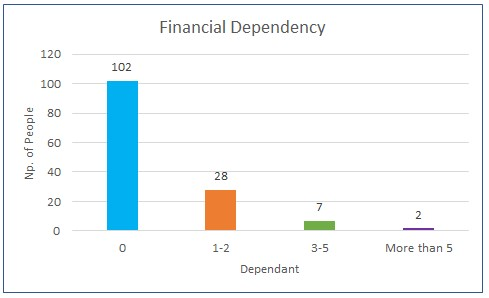
\includegraphics[width=0.8\textwidth]{Images/Finance/Financial Dependency.jpg}
	\caption{Financial dependency}
	\centering
	\label{financialDep}
\end{figure}

\subsubsection{Financial Crisis}
Almost half of the people didn't face any financial trouble during the lockdown. 23 people surveyed did not want to disclose their condition which comprises 17\% of the total. Figure \ref{Crisis}. 

Correlation:
\begin{itemize}
    \item People who had financial problems also faced challenges to maintain their work-life balance
    \item Who had no financial problem also did not take any loan
    \item The indecisive ones here faced hurdles in remote learning and general communication
    \item Those who did not disclose had obstacles in commuting to the workplace
\end{itemize}
\newpage
\begin{figure}[!ht]
	\centering
	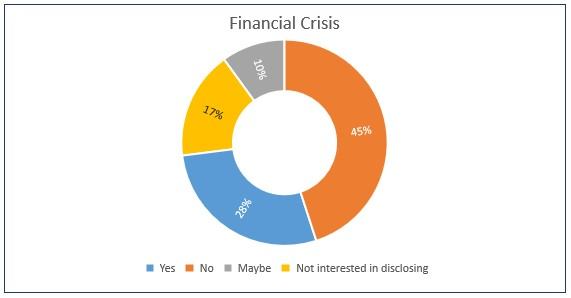
\includegraphics[width=0.8\textwidth]{Images/Finance/Financial Crisis.jpg}
	\caption{Financial crisis}
	\centering
	\label{Crisis}
\end{figure}

\subsubsection{Effect on Overall Income}
From the graph we can see that 74\% of them were detractors in this case that pinpoints the negative condition of them due to the pandemic and 16\% and 10\% were passive and promoter consecutively regarding the matter. It shows the overall financial condition of most of the people was largely affected negatively and they had to face a tough time to cope up. Figure \ref{effct in income}.

\begin{figure}[!ht]
	\centering
	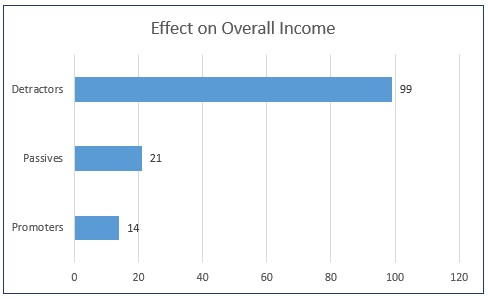
\includegraphics[width=0.8\textwidth]{Images/Finance/Effect on Overall Income.jpg}
	\caption{Effect on overall income}
	\centering
	\label{effct in income}
\end{figure}

\subsubsection{Financial Assistance}
Here we can clearly see that among the people we surveyed almost two-thirds of them didn't receive any financial assistance from their workplace while the rest got the required assistance. Figure \ref{assistance}.

\begin{figure}[!ht]
	\centering
	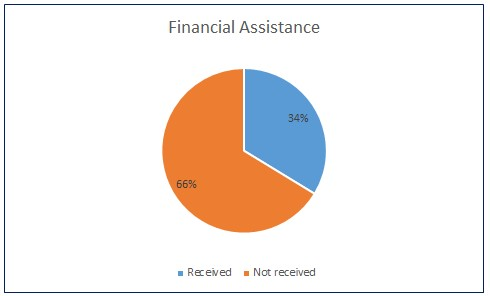
\includegraphics[width=0.8\textwidth]{Images/Finance/Financial Assistance.jpg}
	\caption{Financial assistance}
	\centering
	\label{assistance}
\end{figure}

\subsubsection{Remuneration}
Most of the people received timely remuneration during this pandemic which is a matter of great relief and of great help in times like this. 26 of them faced problems in case of timely remuneration which accounts for almost 23\%. Figure \ref{Remuneration}

\begin{figure}[!ht]
	\centering
	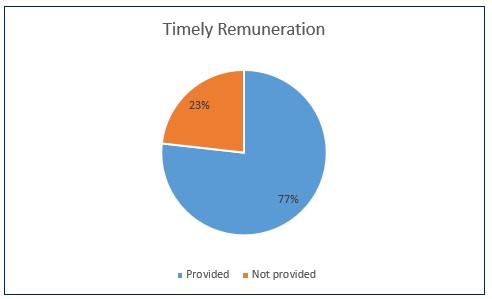
\includegraphics[width=0.8\textwidth, height=2.5in]{Images/Finance/Remuneration.jpg}
	\caption{Remuneration}
	\centering
	\label{Remuneration}
\end{figure}

\subsubsection{Loan}
Most of the people did not have to take any loan to survive through this period which accumulated to 82\% of them. And 12\% of them showed disinterest to disclose the actual scenario which is rather understandable. Figure \ref{Loan}

\begin{figure}[!ht]
	\centering
	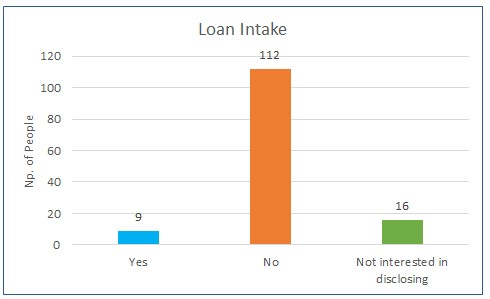
\includegraphics[width=0.8\textwidth]{Images/Finance/Loan.jpg}
	\caption{Loan condition}
	\centering
	\label{Loan}
\end{figure}

\section{Related Works}
Before proceeding with the survey, some back study was necessary to understand the perimeters that should be focused on. Our team studied some relevant works and then we brainstormed the unique ideas on our survey. 
\subsection {Team Communication and Collaboration}
This paper \cite{nafis1} talks about how extensive partnership, collaboration and teamwork among all levels of workers such as scientists, doctors, medical professionals, social workers, policymakers, governments, pharmaceutical firms, and funding aid agencies are needed to stop the pandemic immediately. 

This paper’s \cite{nafis2} goal is to identify opportunities for developing future COVID-19 communication curricula and support tools.
\subsection {Work-Life Balance}
A research team in Berlin, Germany included 1500+ participants from different continents and countries about measuring the stress level and work-life balances in their lives \cite{mishra1}. There were similar patterns regarding lifestyle stresses for participants from Asia, Europe, North America, South America etc. They denoted some factors for first-world countries, while some other factors relating to second-world countries. Difficulties in separating work and family lives, feeling isolated, lack of privacy, as well as over-working, dominated the list of remote working stresses worldwide.

Another team from Indonesia conducted research based on the changes in employees’ lives due to the significant changes in office culture \cite{mishra2}.

\subsection {Work Experience and Environment}
A team in China aimed to describe the experiences of these healthcare providers in the early stages of the outbreak. They conducted the study using an empirical phenomenological approach. Nurses and physicians were recruited from five COVID-19-designated hospitals in Hubei province using purposive and snowball sampling. The study shows that the intensive work drained healthcare providers physically and emotionally \cite{afra1}. Health-care providers showed their resilience and the spirit of professional dedication to overcome difficulties. This may not seem so relevant but the idea of distributing the stress load of the employees and some thoughtful insights helped us to progress in our survey. 


\subsection {Financial}
The paper \cite{saad1} discusses ways to mitigate financial disruption. Some require a political push for more generosity from rich countries, often coupled with financial engineering to maximize impact, while others require reforms in the international economic system that would permit developing countries to mobilize resources by and for themselves.

This paper \cite{saad2} summarises in terms of regional classification, the impact of the outbreak that has been the highest in Asian emerging markets whereas emerging markets in Europe have experienced the lowest.

\section{Limitations}
While conducting the survey, we faced some challenges which led to some biased data sets. Here are some of the limitations mentioned which can be considered for a diversified data set for a future survey.
\begin{itemize}
  \item The majority of the respondents were students doing internships during the time mentioned in the survey.
  \item There were limited data sets due to lack of time to carry out the survey
  \item Non diversified data set as survey form was distributed in a few company 
  \item The survey was conducted in Bangladesh only hence, the result may be biased and not be applicable worldwide.
\end{itemize}

\section{Conclusions and Future Work}
During COVID-19, the work paradigm has shifted greatly and many new variables have been added to the quality of work-life.  Understanding the positive and negative sides of this new paradigm can help us with a smoother transition and gain resilience in the post-COVID-19 era.

In future,  this survey can be extended to a more diversified group of people of varying ages, professions, professional stages and locations. 

%-------------------------------------------------------------------------------
% REFERENCES
%-------------------------------------------------------------------------------
%\newpage
\bibliographystyle{ieeetr}
\bibliography{reference}


\end{document}

